\chapter{Gadolinium Neutron Conversion}
%\label{chap:GdFoil}

%%----------------------------------------------------------------------
%%----------------------------------------------------------------------
%\section{Gadolinium}

%Introduction to Gd
Gadolinium (Gd) is a chemical element with atomic number 64. It is a metal and appears as a solid under standard pressure and room temperature. In nature Gd occurs as a composition of seven isotopes; the most abundant being Gd-158 (24.84\%), followed by Gd-160 (21.86\%), Gd-156 (20.47\%), Gd-157 (15.67\%) and Gd-157 (14.80\%).

%Gd Cross section and its use
Gd has many favorable characteristics allowing an eclectic range of use; for instance in alloys to make magnets, electronics and data storage disks( *); and as a contrast agent in MRI, to diagnose cancerous tumors(*).
Of particular interest is its high neutron absorption cross section, high probability of neutron capture. Of all known natural occurring nuclei, Gd-157 has the highest neutron absorption cross section having resonance at thermal-neutron energies (*). As efficient neutron absorbers, Gd plays an important role in neutron shielding alloys for nuclear reactor safety and storage (*). An additional use of great Gd neutron capture is as Gd-based neutron poison, for instance Gd(III) nitrate in moderator systems for regulating power generation and shut-down of Heavy Water Nuclear Reactors (* page 31).
Not limited to the field of nuclear physics, Gd neutron absorption capability also benefit(s?) neutron capture therapy for cancer treatment and neutron detection, due to reaction products following neutron capture.  In gadolinium neutron capture therapy (GdNCT) a cancer patient is injected with Gd endused tracer followed by exposure to a neutron beam. Neutron absorbed by the Gd tracer produce secondary particles such as photons and electrons. While traversing tissue, the particles deposits dose and The particles travels the tissue exposed to a neutron beam, once Gd absorbs neutrons, decays and release product particles the particles  is injected to the cancer patient product particles deposits dose locally to

%Introduction to neutron detection???

\section{Cross-section}
%Neutron capture in gadolinium
Neutron capture cross section of natural Gd is given by the weighted sum of isotopic cross sections. Relative abundance of Gd isotopes in natural Gd and their neutron capture cross section are listed in table 1. Isotopes Gd-157 and Gd-155 collectively contribute 99.99\% of the cross section, resulting in 48800±150 barns. Natural Gd interaction with thermal neutrons may therefore be simplified as a “two-absorbing isotope system” consisting of the isotopes Gd155 and Gd157 [Dumazert, 2018].

%Nuclear reaction equation ...
\section{Reaction Equation}
Since natural Gd interaction with neutrons can be ascribed to isotopes Gd-157 and Gd-155, it is worth studying their corresponding nuclear reaction equation.

\begin{equation}
    _{64}^{155}Gd \rightarrow _{64}^{156}Gd^* \rightarrow _{64}^{156}Gd + \gamma + ICe^-     (Q=8.5 MeV)
\end{equation}
\begin{equation}
    _{64}^{157}Gd \rightarrow _{64}^{158}Gd^* \rightarrow _{64}^{158}Gd + \gamma + ICe^-    (Q=7.9 MeV)
\end{equation}

Once a Gd nuclei has absorbed a neutron it exists in an excited energy state from which it decays by gamma-transition, resulting primarily in gamma-ray ($\gamma$-ray) emission and internal conversion (IC) electrons. Byproducts of the decay are Auger and Coster-Kronig (ACK) electrons and X-rays, prompted by vacancies left by the IC electrons, for further explanation of gamma-transition see section ??. The Q-value ($Q$) is defines as the difference in mass before and after a nuclear reaction and represents the net energy released when the nuclei has decayed completely. This energy is distributed as kinetic energy among product particles. Due to the Gd nuclei’s large mass, compared to a photon (massless) and an electron, the recoil energy is neglectable ( Modern Nuclear Chemistry, page 219*). I.e. most of the Q-value is distributed among gamma-rays and IC electrons.


\section{Reaction Energy Spectrum}
From Gd(n,gamma) capture, the excitation energy is distributed among reaction products; roughly 99\% of the energy is carried by prompt gamma-rays and the rest by low energy electrons [Sakurai et al.]. The energy spectrum ranges from 0 MeV to the Q-value of the nuclear reaction. Energies of prompt gamma-rays lie all over the spectrum, while energies of IC electrons and their biproducts are mainly located at the lower end, below 0.2 MeV.
The resulting spectrum is an overlap of two basic components. The first is a continuous spectrum, generated by prompt gamma-rays in the medium to high energy range, and the second is a set of discrete lines, produced by low energy prompt gamma-rays, IC electrons, Auger electrons and X-rays. In other words, prompt gamma-ray emission adds to both components, while the remaining reaction products supply just the discrete.

  \begin{figure}[h]
  \centering
  	\includegraphics[width=7cm]{fig/lvl.png}
  	\caption{Nuclear levels of an arbitrary nucleus}
  	\label{fig:1}
  \end{figure}

The spectrums form is closely related to the nuclear structure of gadolinium. Figure ? illustrates excited states of an arbitrary nucleus. A low-lying level has less excitation energy than a high lying level. Low-lying levels are easily distinguishable, each with a known spin and parity, they are discrete. As the excitation energy increases so does the nuclear level density, until high lying levels eventually become indistinguishable from one another and resemble a continuum. In fig. ?, the quasicontinuum domain of energy states is represented by a gradient, where energy level density increases as the gradient darkens. Energy levels within the quasicontinuum are marked by dotted lines and the discrete domain with uninterrupted lines. There is no clear boundary between the continuous and discrete domain, but rather a smooth transition between the two. The highest energy level represents neutron capture state and the lowest level ground state, both are indicated by a bold uninterrupted line. A transition from one level to another is indicated by and arrow.

\subsection{Prompt Gamma-Rays}

A nucleus may transition once or several times before it reaches ground state.
Transitions can occur between (1) states in the continuous domain, (2) states in the discrete domain or (3) between the two. In the continuous domain there are nearly endless possible states from which a nucleus can decay.  It is the transitions with initial states in this domain that bring about the spectrum’s apparent continuity.
In the spectrum, gamma-rays take the form of a broad peak structure along with a couple of prominent spikes. The distribution stretches from one end of the spectrum to the other. The broad peak favors energies in the bottom half of the spectrum, its apex between 0 and 2 MeV, and tapers off slowly as it approaches maximum energy release.

As the nucleus de-excites and gets closer to ground state transitions between states in the discrete domain occurs. There is a limited amount of discrete levels, consequently the number of possible gamma-emission energies are finite, in contrast to the continuum. This results in discrete peaks near the lowest part of the energy spectrum.

\begin{figure}
  \centering
  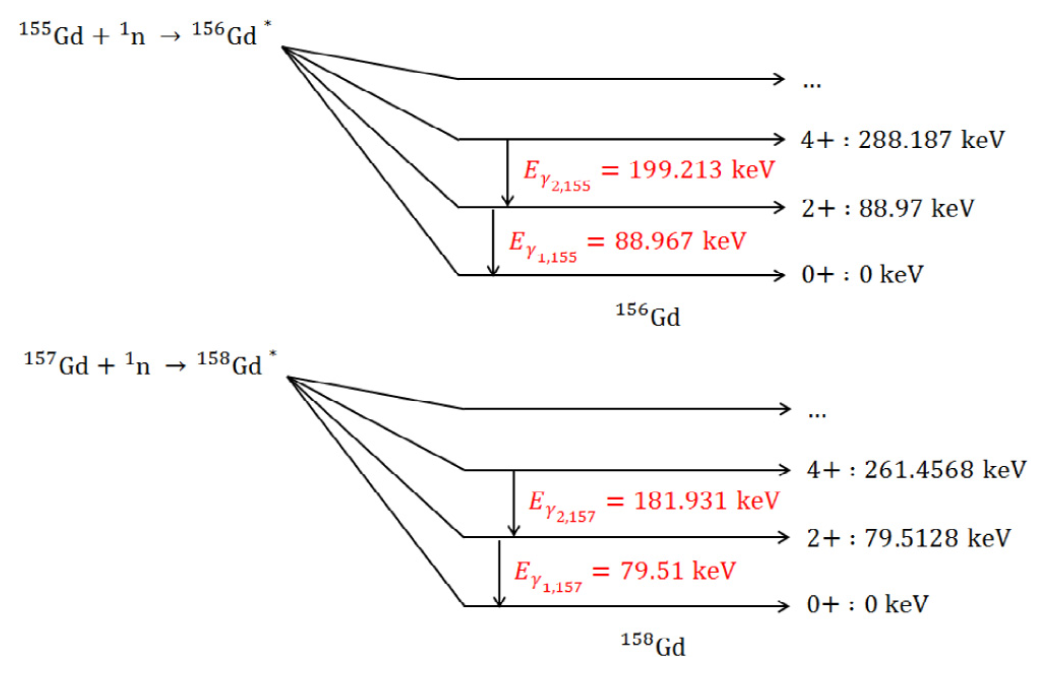
\includegraphics[width=7cm]{fig/Gd_ExcitedStates.png}
  \caption{Excitation levels of Gd-155* and Gd-157* and corrosponding gamma-transitions}
  \label{fig:1}
\end{figure}

Fig. \ref{fig:Gd_ExcitedStates} illustrates gamma-transistions associated with excited gadolinium nuclei. Two peaks, in the lower end, dominate the spectrum. In a purely isotopic material of either Gd-156* or Gd-158* a set of two energy pairs is emitted, {88.97 keV, 199.22 keV} and {79.51 keV, 181.94 keV}, respectively. The lowest energy of each set is characteristic for the transition between first excited state with spin-parity ( J^π)  2$^+$  and ground state 0$^+$, while the larger energy is characteristic for transitions between second excited state with spin-parity 4$^+$ state and first excited state 2$^+$[C.W. Reich, Nuclear Data Sheets for A = 156, Nucl. Data Sheets 113 (11) (2012) 2537–2840.]. Gamma-ray emission rate probability (per neutron capture) of Gd-157 and Gd-155 for are listed in table ?? [Gräfe et. al]

%%----------------------------------------------------------------------
\subsection{Internal Conversion Electrons}
%\textbf{Internal Conversion Electrons}\\
Alternatively, the atom can de-excite by means of internal conversion (IC), the direct emission of an orbital electron. In gadolinium excited by neutron capture, IC is most probable for transitions from first state to ground state $(2^+ \rightarrow 0^+)$ and second state to first state $(4^+ \rightarrow 2^+)$. These transitions are responsible for 96.7\% of the energy carried by IC electrons [??!]. They also happen to be the same transitions from which the discrete gamma-ray duplets, mentioned previously, are produced.

IC and gamma emission are competing decay modes. The ratio of IC decay rate $\lambda_{ICe^-}$ to gamma decay rate $\lambda_{\gamma}$ can be described by the internal conversion coefficient (ICC) $\alpha$:

  \begin{equation}
      \alpha =  \frac{\lambda_{ICe^-}}{\lambda_{\gamma}}
  \end{equation}

In cases where gamma decay is preferred the coefficient is small, perhaps even negligible, and differently when IC is preferred the coefficient is large.

The probability of IC depends on the electron shell (K,L, M, …)and shells therefor have respective coefficients ($\alpha_K$,$\alpha_L$,$\alpha_M$, …).

Inner shell electrons, such as those from the K shell, are more likely to interact directly with the nucleus, since its wavefunction has finite probability of penetrating the nucleus. The probability of IC in a shell becomes less likely the further away it lies from the nucleus. In other words, internal conversion depends heavily on the atomic electron density inside the nucleus. (studie of the probability of IC from shells [ref?], table?). Consequently, odds of nuclear interaction with the K-shell is more likely than with the L-shell, than the M-shell and so on.

The total ICC is the ratio of total number of IC electrons to gamma-rays emitted by a nucleus and it can be expressed as a sum of shell coefficients:

\begin{equation}
    \alpha_{TOT} =  \sum_i \alpha_i \ , \ i = K, L, M, ...
\end{equation}

Transition levels of lower energy favor internal conversion. As calculated by [A.AHarms, Table 4], transitions of Gd-157* from the second lowest transition level, L-shell of the first excited state, are 3 times more likely of mediation by IC than gamma-emission. While de-excitation from higher states are less prone to IC. Already at the third excitation state, Gd-157* exhibits a low coefficient of 0.1, meaning IC electron rates are 10 times lower than gamma rates.

The energy of an IC electron is determined by the available transition energy and the binding energy of a shell.

  \begin{equation}
      E_{ICe^- }=E_T-E_{bi,i},\ , \ i = K, L, M, ...
  \end{equation}

IC electrons contribute to discrete lines in the 20-200 keV range. Eminent is the intensity at which specifically 71 keV electrons are produced, nearly 0.27 nc$^-1$ in natural gadolinium [T.Aoyama].

%%----------------------------------------------------------------------
\subsection{X-rays and Auger Electrons}
When a conversion electron is expelled from subshell m a vacancy is left behind. Still in an excited state, the atom undergoes further de-excitation. An electron from a higher subshell p (>n) descends and fills the vacancy, releasing atomic excitation energy by either emission of x-rays or Auger electrons.
X-ray emission occurs when the transition energy goes into electromagnetic radiation. Difference in binding energy makes up the x-ray energy.

  \begin{equation}
      E_{x-ray} = E_T = E_{bi,p}-E_{bi,m}
  \end{equation}

On the other hand, the transition energy may go into freeing an electron of an intermediate subshell n where n lies between shell m and p. The so-called Auger electron has energy equal to the difference in transition energy and binding energy.

\begin{equation}
    E_{Ae^-} = E_T-E_{bi,n}
\end{equation}

 X-rays and Auger electrons, from L- and K-shell, of gadolinium-neutron capture are radiated in the 0-50 keV range. The most prominent x-ray has energy of 43 keV and an emission rate of 0.47 nc$^-1$ (per neutron capture). Auger electrons worth noting are of energy 35 keV (0.08 nc$^-$) and 5 keV (0.21 nc$^-1$). In comparison to x-rays, they are less frequent and of lower energies. [Dumartez]

%%----------------------------------------------------------------------
%%----------------------------------------------------------------------
